\begin{spacing}{2}
    \section{实验设计}
\end{spacing}
U-Net首次出现在一次医疗图像分割赛事中。U-Net基于全卷积网路,使用对称结构并且在小数据集表现优异。

遥感图像和医疗图像的共同之处在于,数据集小、尺寸巨大。可以说,应用在医疗图像上的U-Net为我们提供了对遥感图像进行分割的重要思路。

本章主要介绍了数据集的选择及处理、卷积核的初始化方案以及对生成图像的优化方案。

\subsection{数据集选择及处理}
这次选择的数据集是Inria Aerial Image Labeling Dataset\cite{maggiori2017dataset}。数据集的原始图像大小为$5000\times 5000$,共计180组遥感图像。每组图像含1张3通道遥感图像和1张单通道ground-truth。样例如图\ref{Fig:sample_dataset}。

\begin{figure}[htbp]
    \centering
    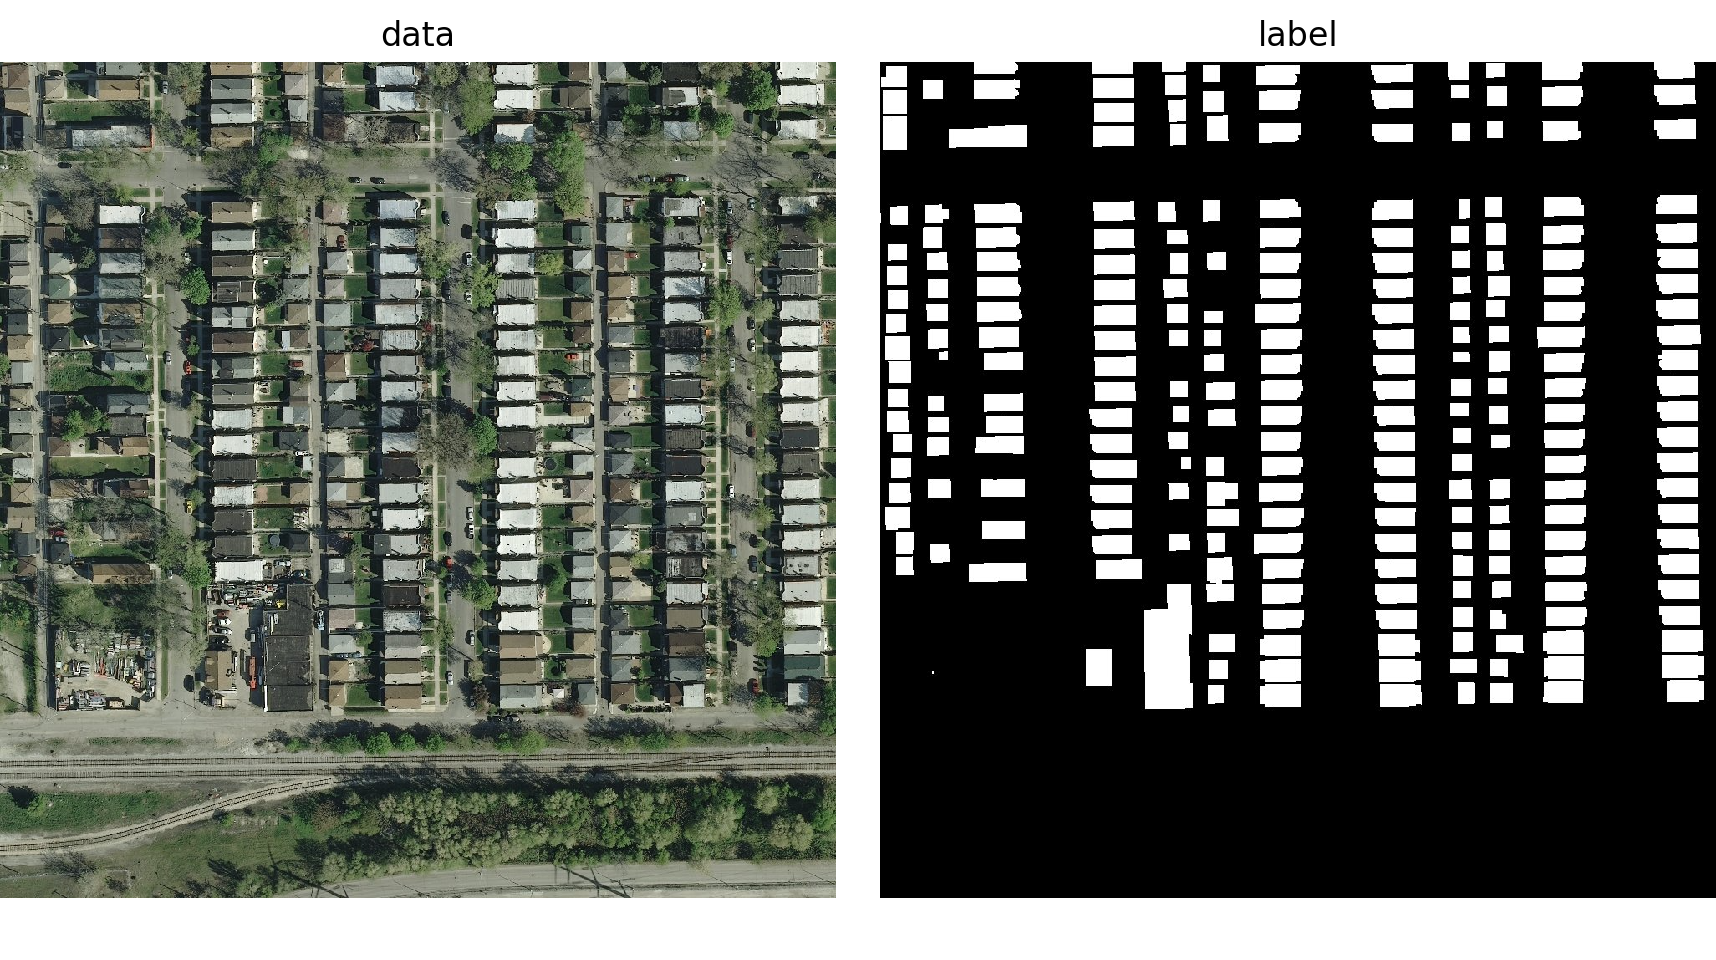
\includegraphics[width=1\textwidth]{Figures/sample_dataset.png}
    \caption{数据集样例图}
    \label{Fig:sample_dataset}
    
\end{figure}

此次训练使用小批量梯度下降法。由于显存限制,经过测试,$500\times 500$左右大小的图像mini batch size只能设置为1。如果每次只训练一张的话,会陷入局部最优解。如果输入图像大小在$250\times 250$左右的话,mini batch size 可以设置为4。

由于池化核的大小为$2\times 2$,因此输入图像的大小最好是2的整次方。最终确定将图像切割为$256\times 256$。原图尺寸大小为$5000\times 5000$,因此将原图调整大小至$4864\times 4864$大小之后再进行分割。这个大小是256的19倍,并且对原图损失不大。这样共得到了64980张图像。由于数据集本身已经够大,因此不再做数据拓展。

得到的$256\times 256$的图像还要分离特征。由于ground-truth为单通道图像,取值为0处为非建筑,取值为255处为建筑,因此我们将图像变换为$256\times 256\times 2$的张量。像素点处取值为0的点取值为$[1,0]$,像素点处取值为255的点取值为$[0,1]$。

此次训练数据集共有六万多组,数据为$246\times 256$的3通道图像和$256\times 256\time 2$的张量,单张图像也很大,因此训练的性能是十分重要的。在训练时以二进制文件格式读入将会对性能产生重大影响,从而影响模型的训练时间。使用二进制数据再磁盘上占用的空间更少,复制时间更短。TFRecord是TensorFlow自己的二进制存储格式,针对TensorFlow以多种方式进行了优化,可以轻松组合多个数据集。因此将得到的矩阵与原图像打包成180组TFRecord数据送入神经网络。
\subsection{图像处理流程设计}
\subsubsection{网络结构}
初始的U-Net网络结构如图\ref{Fig:unet_construction}所示。

\begin{figure}[htbp]
    \centering
    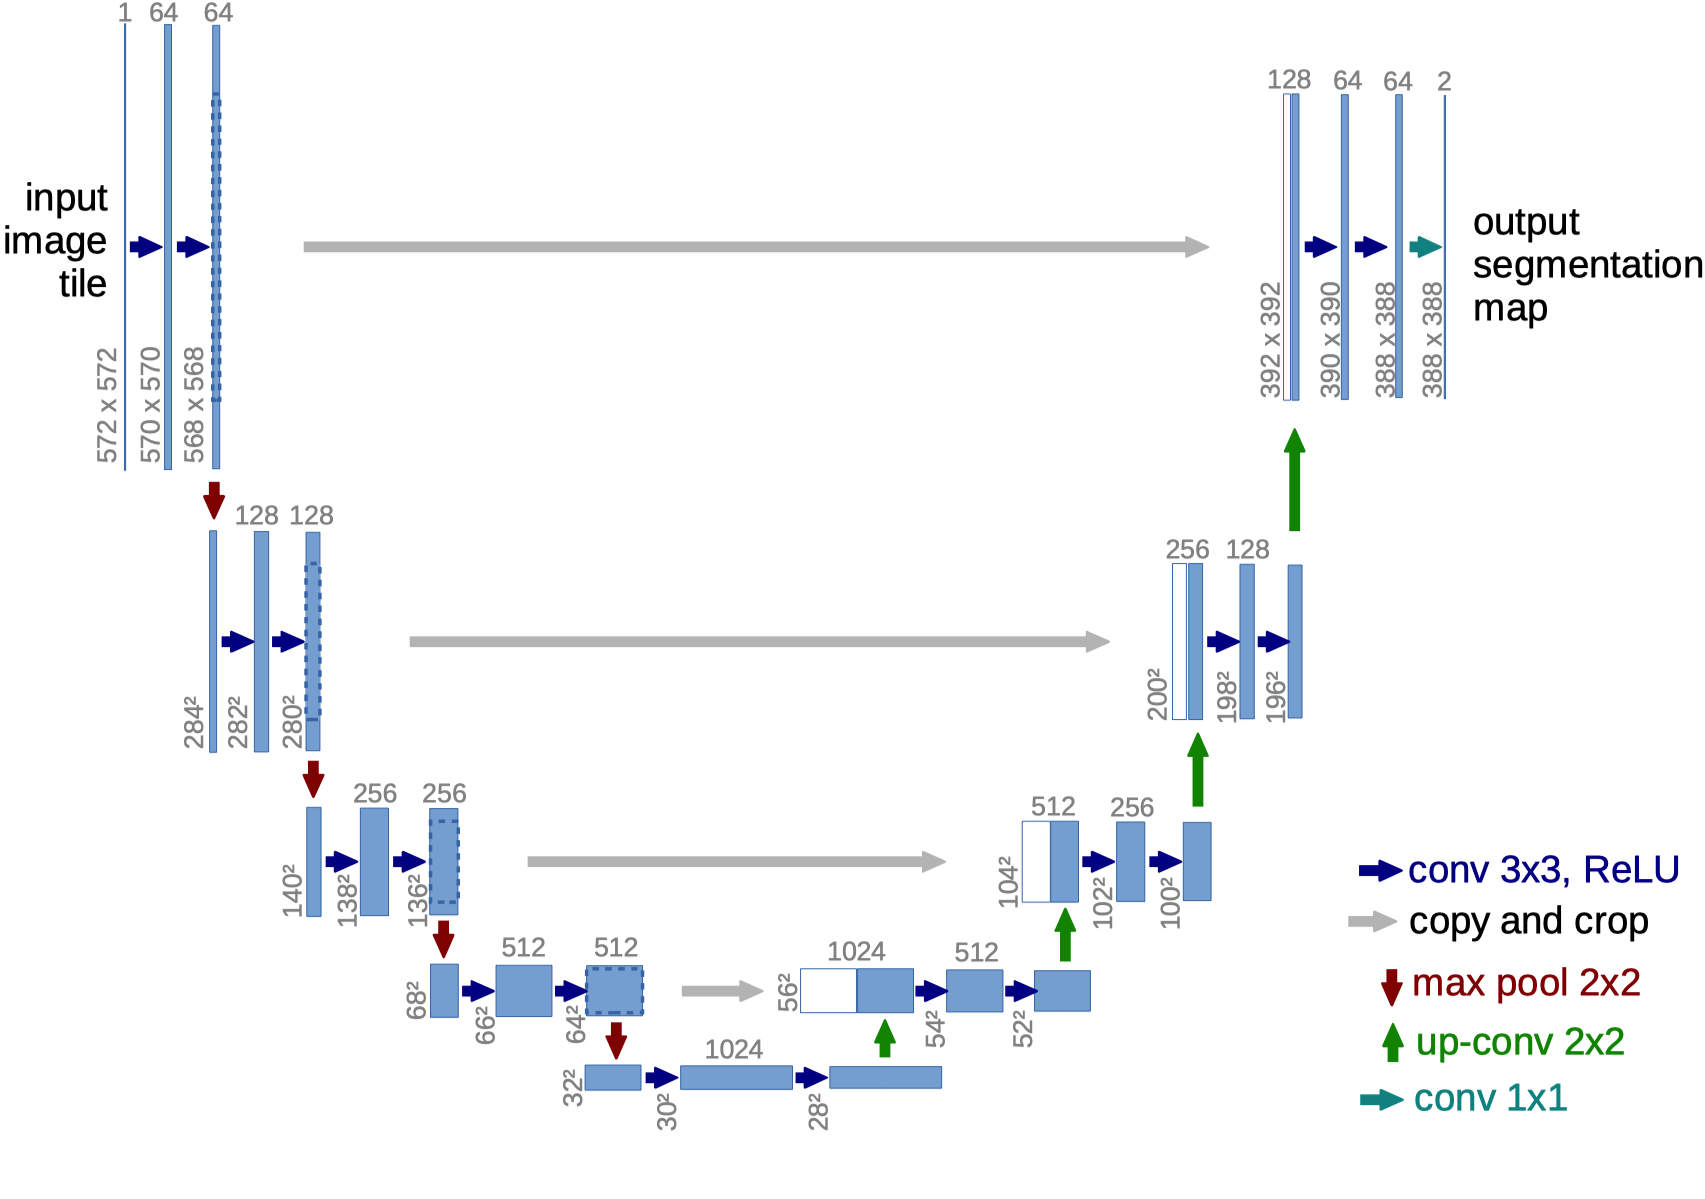
\includegraphics[width=1\textwidth]{Figures/unet_construction.png}
    \caption{U-Net网络结构(来源\cite{ronneberger2015u})}
    \label{Fig:unet_construction}
    
\end{figure}

网络分为收缩路径和扩张路径两部分。该示意图的左边为收缩路径,该示意图的右边为扩张路径。在收缩路径中,每使用$3\times 3$大小的卷积核进行两次卷积运算之后就进行一个大小为$2\times 2$的最大池化来下采样。卷积核的激活函数使用ReLU函数。每次下采样之后图像的特征长度就翻一倍。在进行4次最大池化之后再进行两次卷积操作开始上采样,进入扩张路径。在扩张路径中,首先进行反卷积。将反卷积之后的结果与收缩路径中在宽度和高度维度上差不多大小的卷积层进行拼接。再将拼接的结果一起进行卷积核大小为$3\times 3$的卷积。每进行两次卷积就进行一个反卷积使输出的图像长宽变为原来的两倍,面积变为原来的4倍。与此同时,特征数量也减少至原来的一半。在扩张路径中,卷积层使用的激活函数同样也是ReLU激活函数。最终得到的输出再与一个卷积核为$1\times 1$的卷积层相连接。将特征维度长度为64的特征映射到一个长度为2的向量。该向量表示的就是该位置的像素点属于某一类别的概率。

论文\cite{ronneberger2015u}中使用valid卷积方式。论文中的输入图像带下为$572\times 572$像素,经过该卷积神经网络之后得到的输出图大小为$388\times 388$,两者差距不大,因此可以通过插值方法将两张图像调整至同一大小计算损失函数。但是经过计算,$256\times 256$大小的图像在通过U-Net网络后,输出图像大小为$68\times 68$,与原图像大小相差太大,不好与ground-truth计算交叉熵。因此在这里选用same卷积方式,这样输出图像大小仍为$256\times 256$。

\subsubsection{卷积核初始化方案}
在试验中尝试了三种卷积核初始化方案。

\begin{enumerate}
    \item 将卷积核初始化为均值为0,标准化为0.1的正态分布;
    \item MSRA初始化\cite{he2015delving}方法;
    \item Xavier初始化\cite{glorot2010understanding}方法。
\end{enumerate}

MSRA方法来自He等人的论文\cite{he2015delving},其将卷积核初始化进行均值为0,方差为$\sqrt{\frac{2}{n}}$的高斯分布,其中$n$为该卷积核参数的个数。

Xavier初始化方法来自论文\cite{glorot2010understanding}。其主要思想是将参数初始化为$[-\sqrt{\frac{6}{n^k+n^{k+1}}},\sqrt{\frac{6}{n^k+n^{k+1}}}]$范围内的均匀分布,其中$k$为网络的层数,$n$为卷积核参数的个数。

经过试验,前两种方法在训练到100轮左右,交叉熵为0.6左右的时候会陷入局部最优,生成全黑的图像。因此在正式训练的时候采用Xavier初始化方法。

\subsubsection{输出图像恢复及优化}
卷积神经网络输出的图像是$256\times 256\times 2$的以浮点形式存储的张量。首先需要比较每一个像素点处较大的数所处的通道,将输出的矩阵恢复成$256\times 256\times 2$的特征矩阵。然后根据色彩表,将输出矩阵恢复为$256\times 256$大小的单通道图像。

在之前的论文中有人使用条件随机场对生成的图像做更精准的切分,如\cite{chandra2016fast}中,这里时间有限就没有做这种尝试。本次实验使用了开运算。开运算指的是先对图像进行腐蚀操作,再对图像进行膨胀操作的图像处理方法。开运算可以用来消除小物体,在纤细点出分离物体,在平滑较大物体的边界同时并不明显改变其面积。腐蚀操作可以让图像的边界朝内部进行收缩。这种方法还可以消除边界点。一般用来去除图像中小且没有意义的物体。腐蚀操作首先使用结构元素从左上角至右下角逐一扫描图像上的每一个像素。这种结果元素通常是大小为$n\times n$大小的矩形。结构元素覆盖的区域与该结构元素做与运算。如果结果都为1,则该像素为1,如果都为0,则该像素取0。膨胀操作是另外一种图像形态学处理方法。其效果是使物体的边界向外部扩张,让与物体接触的背景点合并到该物体中去。这种方法可以用来填补物体中的空洞。膨胀操作与腐蚀操作一样,使用结构元素逐像素从左上角至右下角扫描图像。将结构元素与与其覆盖的图像做与操作,如果都为0,使该像素为0,否则为1。

此次试验使用了$3\times 3$大小的结构元素和$5\times 5$大小的结构元素分别做了测试,结果是$3\times 3$的结构元素较$5\times 5$的结构元素效果好。

\subsection{损失设计}
原始的U-Net网络论文中损失使用的是交叉熵加上一些正则化项。此次试验除了交叉熵之外,还设计使用类别平衡交叉熵作为损失函数。

使用交叉熵之前,都先对卷积网络输出图像进行逻辑回归。分类网络中使用的回归方法主要是Softmax回归。该回归方法是logistic回归模型的拓展。logistic回归模型只能解决二分类问题,而Softmax回归模型可以解决多分类问题。虽然此次的数据集只标注了建筑和非建筑,但是为了使代码具有通用性,还是使用了Softmax回归方法以使其能够应对未来可能遇到的多分类问题。
\begin{equation}\label{softmax}
    p_k(x)=\exp(\frac{a_k(x)}{\sum\limits_{k'=1}^K \ \exp(a_{k'}(x))})
\end{equation}

公式\ref{softmax}中$K$是分割类别数,$k\in K$。具体到这个数据集来说,类别分为建筑和非建筑,因此$K=2$。

$\mathbb{Z}^2$为全体像素集合,$x\in \mathbb{Z}^2$。$a_k(x)$即在$x$处类别$k$的取值。
\subsubsection{交叉熵}
\begin{equation}
    Loss=-\sum\limits_{i=1}^n\ p(y\__i)\cdot \log(p(y_i))
\end{equation}
交叉熵一般用来表示目标与预测值之间的差距。当使用神经网络进行分类和预测时,交叉熵误差较分类误差和均方误差来说,能更好地评估神经网络的质量。在分类问题中,交叉熵函数曲线是一个凸函数,便于使用梯度下降法进行反向传播,因此针对分类问题一般采用交叉熵函数作为损失函数。
\subsubsection{带权重的交叉熵}
我们也常会遇到样本不平衡的问题。为了解决样本不均衡的问题我们通常采取过采样少数类、降采样多数类和调整类权重等方法。在本次实验中,我选择采取调整类权重的方法。

对于城市的遥感图像,建筑占比较大,但是在乡村的遥感图像,建筑占比很小。如果我们单纯使用交叉熵函数作为损失函数的话,很有可能在乡村的遥感图像中漏报建筑。因此使用带权重的交叉熵,增加少数类分错的权重是很有必要的。
\begin{equation}\label{entropy}
    Loss=-\sum\limits_{i=1}^n\ \alpha_i\cdot p(y\__i)\cdot \log(p(y_i))
\end{equation}
\subsubsection{类别平衡交叉熵}
\begin{equation}\label{class_balanced_cross_entropy}
    \begin{aligned}
        Loss= & -\beta\cdot p(y_-\in Y_+)\cdot \log(p(y\in Y+))      \\
              & -(1-\beta)\cdot p(y_-\in Y_-)\cdot \log(p(y\in Y_-))
    \end{aligned}
\end{equation}

在\cite{xie2015holistically}中提出了一种被称为类别平衡交叉熵函数的方法计算损失。因为边缘像素的数量远远小于非边缘像素的数量,因此在训练时容易陷入向全取非边缘像素方向的局部最优。使用这种方法可以自动取得权重。遥感图像中既有城市的遥感图像也有乡村的遥感图像,因此取固定权重也不是一个好方法。如果使用类别平衡交叉熵的话可以自动计算权重,能够更好地适应城市和乡村两种不同的遥感图像。

公式\ref{class_balanced_cross_entropy}中引入了一个像素级的类别平衡权重$\beta$,其值是被标记为建筑的像素占所有像素的比值:
\begin{equation}
    \beta=\frac{|Y_-|}{|Y|}
\end{equation}
这实际上也是一种带权重的交叉熵,只不过该交叉熵的权重是自动计算得到的。
\subsection{结果评估}
每次迭代均会计算混淆矩阵,利用混淆矩阵计算准确率(Accuracy)、精确率(Precision)、召回率(Recall)和F1 Score。同时还会计算预测结果与ground-truth之间的交叉熵。

\begin{table}[htbp]
    \centering
    \caption{混淆矩阵}
    \label{Tab:confusion_matrix}
    \begin{tabular}{|c|c|c|c|}
        \hline
                                & \multicolumn{2}{c|}{真实值} & 总数              \\
        \hline
        \multirow{2}*{预测输出} & 真阳性(TP)                & 伪阳性(FP) & P' \\
        \cline{2-4}
                                & 伪阴性(FN)                & 真阴性(TN) & N' \\
        \hline
        总数                    & P                           & N            &    \\
        \hline
    \end{tabular}
    
\end{table}
表\ref{Tab:confusion_matrix}为混淆矩阵。真阳性的意思是在预测中正样本预测正确的数量;伪阳性的意思是在预测中正样本预测错误的数量;伪阴性的意思是在预测中负样本预测错误的数量;真阴性的意思是在预测中负样本预测正确的数量。

准确率指的是预测输出中分类正确的样本数占总样本的比值,使用\ref{accuracy}计算:
\begin{equation}\label{accuracy}
    Accuracy=\frac{TP+TN}{P+N}
\end{equation}

精确率指的是真阳性占预测输出中阳性样本的比值,使用\ref{precision}计算:
\begin{equation}\label{precision}
    Precision=\frac{TP}{TP+FP}
\end{equation}

召回率指的样本中的阳性样本被正确预测占所有阳性样本的比值,使用\ref{recall}计算:
\begin{equation}\label{recall}
    Recall=\frac{TP}{TP+FN}
\end{equation}

F1 Score是精确率和召回率的调和均值,使用\ref{f1-score}计算:
\begin{equation}\label{f1-score}
    F_1=\frac{2\cdot Precision\cdot Recall}{Precision+Recall}
\end{equation}
\subsection{具体实现}
\subsubsection{实验平台}
本次实验训练使用Anaconda版Python 3.7下的TensorFlow-GPU 1.8。后期图像生成由于GPU显存限制,使用TensorFlow的CPU版本进行计算预测图计算。
\subsubsection{模型实现}
此次试验的源代码托管于GitHub仓库gzr2017/UNet-AerialImageSegmentation中,主要文件及作用如表\ref{Tab:file_list}。
\begin{table}[htbp]
    \centering
    \caption{文件列表}
    \label{Tab:file_list}
    \scalebox{1.0}{
        \begin{tabular}{cc}
            \toprule  %添加表格头部粗线
            文件名   & 作用                                           \\
            \midrule  %添加表格中横线
            utils.py & 实现了基础的图像分割、合并、分离通道及命名工具 \\
            data.py  & 实现了生成数据集及图像存放目录工具             \\
            model.py & 定义网络结构                                   \\
            cnn.py   & 定义网络的损失函数、评估函数及预测方法         \\
            train.py & 定义了网络训练方法                             \\
            \hline \hline
        \end{tabular}
    }
    
\end{table}
